\documentclass[11pt]{article}

\usepackage[margin=1in]{geometry}
\usepackage{graphicx}
\usepackage{array}
\usepackage{longtable}
\usepackage{hyperref}
\usepackage{booktabs}
\usepackage{xcolor}
\usepackage{tikz}
\usepackage{float}
\usepackage{enumitem}
\usepackage{fancyhdr}
\usepackage{titlesec}
\usepackage{tcolorbox}
\usepackage{tabularx}
\usepackage{multirow}
\usepackage{caption}
\usepackage{subcaption}

\usetikzlibrary{shapes.geometric, arrows.meta, positioning, fit, backgrounds, calc}

% Color definitions
\definecolor{sudcolor}{RGB}{70,130,180}
\definecolor{actorcolor}{RGB}{60,179,113}
\definecolor{systemcolor}{RGB}{255,165,0}
\definecolor{devicecolor}{RGB}{186,85,211}
\definecolor{flowcolor}{RGB}{100,100,100}
\definecolor{sectionblue}{RGB}{31,78,121}
\definecolor{lightgray}{RGB}{245,245,245}
\definecolor{warningred}{RGB}{220,53,69}
\definecolor{successgreen}{RGB}{40,167,69}

% Hyperref setup
\hypersetup{
    colorlinks=true,
    linkcolor=sectionblue,
    urlcolor=sectionblue,
    citecolor=sectionblue
}

% Header and footer
\pagestyle{fancy}
\fancyhf{}
\fancyhead[L]{\leftmark}
\fancyhead[R]{Context Diagram Documentation}
\fancyfoot[C]{\thepage}
\renewcommand{\headrulewidth}{0.4pt}
\renewcommand{\footrulewidth}{0.4pt}

% Section formatting
\titleformat{\section}
  {\normalfont\Large\bfseries\color{sectionblue}}{\thesection}{1em}{}
\titleformat{\subsection}
  {\normalfont\large\bfseries\color{sectionblue!80}}{\thesubsection}{1em}{}
\titleformat{\subsubsection}
  {\normalfont\normalsize\bfseries\color{sectionblue!60}}{\thesubsubsection}{1em}{}

% Custom box environments
\newtcolorbox{keypoint}{
    colback=blue!5,
    colframe=sectionblue,
    title=Key Point,
    fonttitle=\bfseries
}

\newtcolorbox{warning}{
    colback=red!5,
    colframe=warningred,
    title=Warning,
    fonttitle=\bfseries
}

\newtcolorbox{bestpractice}{
    colback=green!5,
    colframe=successgreen,
    title=Best Practice,
    fonttitle=\bfseries
}

\newtcolorbox{example}{
    colback=lightgray,
    colframe=flowcolor,
    title=Example,
    fonttitle=\bfseries
}

\title{%
    \vspace{-1cm}
    \textbf{\Huge Software Architecture Documentation}\\[12pt]
    \Large Context Diagram View\\[8pt]
    \large A Comprehensive Guide to System Boundary Definition\\
    and External Interface Documentation
}
\author{%
    \textit{Architecture Documentation Series}\\[4pt]
    \small Based on IEEE 42010, ISO/IEC/IEEE 12207, and Industry Best Practices
}
\date{\today}

\begin{document}

\maketitle
\thispagestyle{empty}

\vspace{1cm}

\begin{abstract}
\noindent
The Context Diagram is a fundamental architectural view that defines the boundary between a system under design and its external environment. This document provides comprehensive guidance for creating effective context diagrams, documenting external entities and their interactions, and establishing clear system boundaries. The context diagram serves as a critical communication tool among stakeholders, providing a high-level understanding of system scope, external dependencies, and integration points. This guide covers theoretical foundations, practical methodologies, notation standards, quality attribute considerations, and common patterns for various system types including enterprise applications, embedded systems, cloud-native architectures, and distributed systems.
\end{abstract}

\vfill

\begin{center}
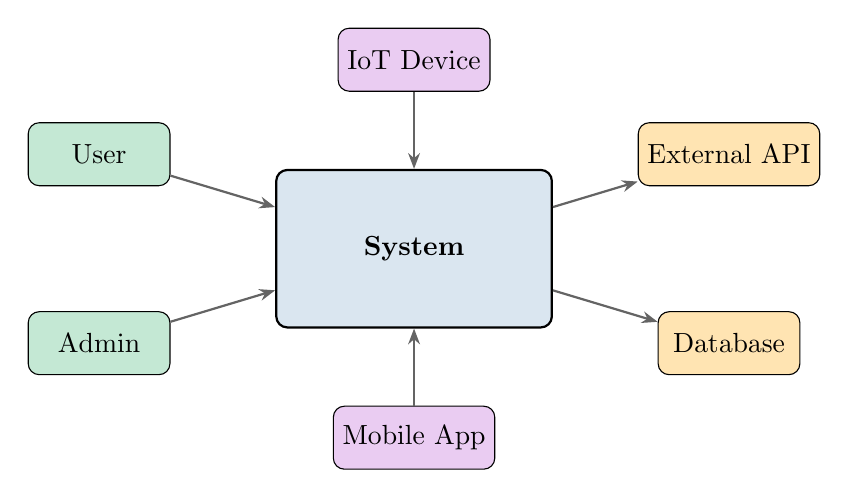
\begin{tikzpicture}[
    scale=0.8,
    actor/.style={draw, fill=actorcolor!30, minimum width=1.8cm, minimum height=0.8cm, rounded corners},
    system/.style={draw, fill=systemcolor!30, minimum width=1.8cm, minimum height=0.8cm, rounded corners},
    sud/.style={draw, thick, fill=sudcolor!20, minimum width=3.5cm, minimum height=2cm, rounded corners},
    device/.style={draw, fill=devicecolor!30, minimum width=1.8cm, minimum height=0.8cm, rounded corners},
    flow/.style={-{Stealth[length=2mm]}, thick, flowcolor}
]
    \node[sud] (sud) at (0,0) {\textbf{System}};
    \node[actor] (user1) at (-5,1.5) {User};
    \node[actor] (user2) at (-5,-1.5) {Admin};
    \node[system] (ext1) at (5,1.5) {External API};
    \node[system] (ext2) at (5,-1.5) {Database};
    \node[device] (dev1) at (0,3) {IoT Device};
    \node[device] (dev2) at (0,-3) {Mobile App};
    
    \draw[flow] (user1) -- (sud);
    \draw[flow] (user2) -- (sud);
    \draw[flow] (sud) -- (ext1);
    \draw[flow] (sud) -- (ext2);
    \draw[flow] (dev1) -- (sud);
    \draw[flow] (dev2) -- (sud);
\end{tikzpicture}
\end{center}

\newpage
\tableofcontents
\newpage

%==============================================================================
\section{Introduction to Context Diagrams}
%==============================================================================

\subsection{Definition and Purpose}

A context diagram represents the highest level of abstraction in system documentation, depicting the system under design (SUD) as a single process or ``black box'' that interacts with external entities in its environment. The primary purposes of a context diagram are as follows. First, the diagram establishes clear boundaries by defining precisely what is inside and outside the system scope, eliminating ambiguity about system responsibilities. Second, it identifies stakeholders by documenting all external actors, systems, and devices that interact with the system. Third, it maps integration points by showing the high-level data flows, control flows, events, and messages exchanged between the system and its environment. Fourth, it provides communication by serving as a shared reference for technical and non-technical stakeholders to understand the system's place within the broader ecosystem. Fifth, it serves as a foundation, providing the basis for more detailed architectural views, requirements traceability, and interface specifications.

The context diagram answers fundamental questions about the system. What are the boundaries of the system? Who and what interacts with the system? What information flows into and out of the system? What external dependencies does the system have? What are the trust boundaries?

\subsection{Historical Background and Standards}

The context diagram concept emerged from structured analysis methodologies developed in the 1970s, particularly through the work of Tom DeMarco and Edward Yourdon. In data flow diagram (DFD) hierarchies, the context diagram represents ``Level 0,'' showing the entire system as a single process. Modern architectural frameworks have adapted and extended this concept.

The IEEE 42010 standard (Systems and Software Engineering---Architecture Description) provides a framework for architectural views and viewpoints. Context diagrams align with the ``Context Viewpoint'' that addresses how the system relates to its environment. ISO/IEC/IEEE 12207 (Software Life Cycle Processes) recognizes context definition as essential to architectural design. The C4 Model developed by Simon Brown explicitly includes a ``System Context Diagram'' as the first level of architectural documentation. TOGAF (The Open Group Architecture Framework) incorporates context diagrams within its Architecture Development Method (ADM).

\subsection{Relationship to Other Architectural Views}

The context diagram does not exist in isolation but serves as the foundation for a hierarchy of increasingly detailed architectural views.

\begin{figure}[H]
\centering
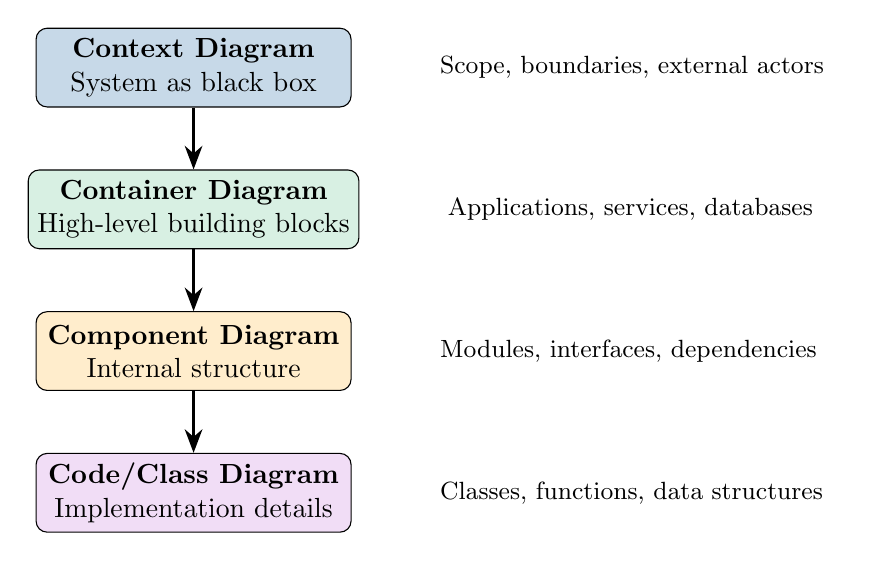
\begin{tikzpicture}[
    scale=0.9,
    box/.style={draw, rounded corners, minimum width=4cm, minimum height=1cm, align=center},
    arrow/.style={-{Stealth[length=3mm]}, thick}
]
    \node[box, fill=sudcolor!30] (ctx) at (0,4) {\textbf{Context Diagram}\\System as black box};
    \node[box, fill=actorcolor!20] (cont) at (0,2) {\textbf{Container Diagram}\\High-level building blocks};
    \node[box, fill=systemcolor!20] (comp) at (0,0) {\textbf{Component Diagram}\\Internal structure};
    \node[box, fill=devicecolor!20] (code) at (0,-2) {\textbf{Code/Class Diagram}\\Implementation details};
    
    \draw[arrow] (ctx) -- (cont);
    \draw[arrow] (cont) -- (comp);
    \draw[arrow] (comp) -- (code);
    
    \node[right=1cm of ctx, text width=5cm, font=\small] {Scope, boundaries, external actors};
    \node[right=1cm of cont, text width=5cm, font=\small] {Applications, services, databases};
    \node[right=1cm of comp, text width=5cm, font=\small] {Modules, interfaces, dependencies};
    \node[right=1cm of code, text width=5cm, font=\small] {Classes, functions, data structures};
\end{tikzpicture}
\caption{Architectural View Hierarchy}
\end{figure}

The context diagram informs requirements engineering by validating scope and identifying interface requirements. It provides essential input to system decomposition by establishing what must be decomposed. It guides deployment architecture by identifying external integration points. It supports security architecture by establishing trust boundaries. Finally, it enables test planning by defining system-level test boundaries.

%==============================================================================
\section{System Boundary Definition}
%==============================================================================

\subsection{Principles of Boundary Definition}

Defining the system boundary is one of the most critical and consequential architectural decisions. A well-defined boundary provides development focus by creating a clear scope for design, implementation, and testing. It enables responsibility assignment through an unambiguous delineation of who is responsible for what. It supports contract definition at integration points where interface contracts can be established. It establishes cost boundaries for estimation and project planning. Finally, it defines risk scope by bounding what can affect the system's quality attributes.

\begin{keypoint}
The system boundary should be stable throughout the development lifecycle. Frequent boundary changes indicate insufficient requirements analysis or stakeholder alignment. Changes to the boundary typically require re-evaluation of scope, schedule, and budget.
\end{keypoint}

\subsection{Boundary Documentation Template}

The following template provides a structured approach to documenting system boundaries:

\begin{tcolorbox}[colback=lightgray, colframe=flowcolor, title=System Boundary Specification]
\textbf{System Under Design (SUD):}\\
Provide the official system name and version identifier.

\vspace{0.3cm}
\textbf{System Mission Statement:}\\
A concise statement (1-2 sentences) describing the system's primary purpose and value proposition.

\vspace{0.3cm}
\textbf{In-Scope Elements:}
\begin{itemize}[nosep]
    \item Functional capabilities the system provides
    \item Data the system owns and manages
    \item User interfaces the system presents
    \item APIs and services the system exposes
    \item Processing and business logic the system executes
\end{itemize}

\vspace{0.3cm}
\textbf{Out-of-Scope Elements:}
\begin{itemize}[nosep]
    \item Functionality explicitly excluded from this system
    \item Data owned by external systems
    \item Processing delegated to external services
    \item User interfaces provided by other systems
    \item Capabilities deferred to future releases
\end{itemize}

\vspace{0.3cm}
\textbf{Boundary Rationale:}\\
Document the reasoning behind boundary decisions, including business constraints, technical limitations, organizational factors, and stakeholder agreements.
\end{tcolorbox}

\subsection{Scope Categories}

When documenting scope, consider these categories:

\subsubsection{Functional Scope}
Functional scope addresses what the system does. This includes business processes supported or automated, features and capabilities provided, data processing and transformations performed, and decision logic and rules implemented.

\subsubsection{Data Scope}
Data scope addresses what information the system manages. This includes data entities owned by the system (system of record), data entities referenced from external sources, data retention and lifecycle policies, and data quality responsibilities.

\subsubsection{User Scope}
User scope addresses who the system serves. This includes primary users and their roles, secondary users and stakeholders, administrative and operational users, and automated actors and agents.

\subsubsection{Technical Scope}
Technical scope addresses what technology the system encompasses. This includes infrastructure components, middleware and runtime platforms, development and deployment tools, and monitoring and management capabilities.

\subsection{Boundary Anti-patterns}

\begin{warning}
Avoid these common boundary definition mistakes:

\textbf{Scope Creep:} Gradually expanding boundaries without formal change control leads to schedule overruns and architectural drift.

\textbf{Fuzzy Boundaries:} Ambiguous phrases like ``as needed'' or ``if time permits'' create implementation confusion and quality risks.

\textbf{Overlapping Boundaries:} Multiple systems claiming ownership of the same functionality or data creates integration nightmares.

\textbf{Premature Optimization:} Excluding functionality to reduce scope without understanding impact on system coherence.

\textbf{Political Boundaries:} Defining scope based on organizational politics rather than technical and business factors.
\end{warning}

%==============================================================================
\section{Context Diagram Notation and Conventions}
%==============================================================================

\subsection{Visual Notation Standards}

While no single notation standard dominates context diagram representation, consistency within an organization is essential. The following notation conventions are widely recognized and recommended:

\subsubsection{System Under Design (SUD) Representation}

The SUD should be visually prominent, typically centered in the diagram. Common representations include a large rectangle or rounded rectangle, a process symbol (circle in DFD notation), or a box with a distinctive border or fill color. The SUD should be labeled with the official system name and optionally include a brief descriptor or version.

\begin{figure}[H]
\centering
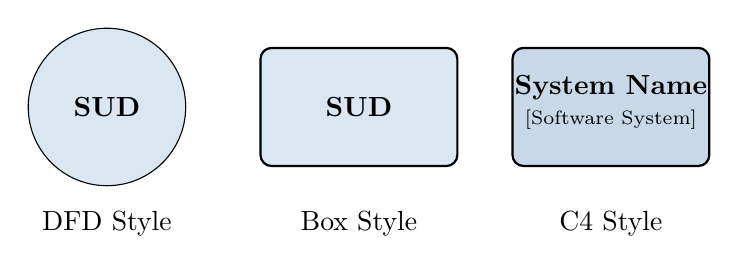
\begin{tikzpicture}[scale=0.8]
    % DFD Style
    \node[draw, circle, minimum size=2cm, fill=sudcolor!20] at (-4,0) {\textbf{SUD}};
    \node[below] at (-4,-1.5) {DFD Style};
    
    % Box Style
    \node[draw, thick, minimum width=2.5cm, minimum height=1.5cm, fill=sudcolor!20, rounded corners] at (0,0) {\textbf{SUD}};
    \node[below] at (0,-1.5) {Box Style};
    
    % C4 Style
    \node[draw, thick, minimum width=2.5cm, minimum height=1.5cm, fill=sudcolor!30, rounded corners] (c4) at (4,0) {};
    \node at (4,0.3) {\textbf{System Name}};
    \node[font=\scriptsize] at (4,-0.2) {[Software System]};
    \node[below] at (4,-1.5) {C4 Style};
\end{tikzpicture}
\caption{Common SUD Representation Styles}
\end{figure}

\subsubsection{External Entity Representation}

External entities should be visually distinguished by type. The recommended approach uses different shapes or colors for different entity categories:

\begin{figure}[H]
\centering
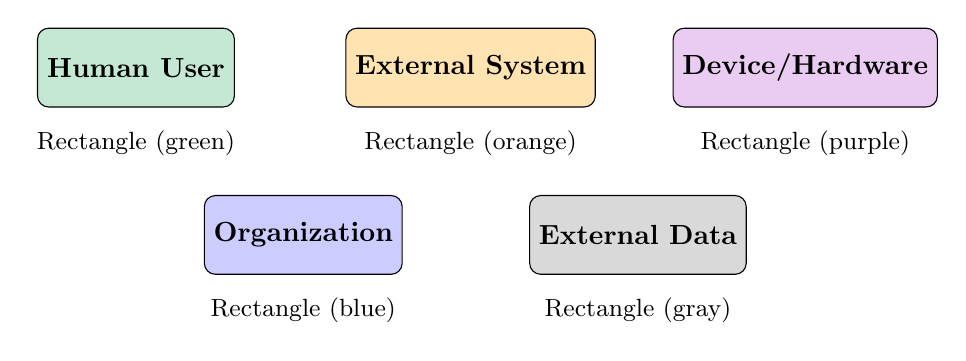
\begin{tikzpicture}[scale=0.85]
    % Human Actor
    \node[draw, fill=actorcolor!30, minimum width=2.5cm, minimum height=1cm, rounded corners] at (-5,2) {\textbf{Human User}};
    \node[below, font=\small] at (-5,1.2) {Rectangle (green)};
    
    % External System
    \node[draw, fill=systemcolor!30, minimum width=2.5cm, minimum height=1cm, rounded corners] at (0,2) {\textbf{External System}};
    \node[below, font=\small] at (0,1.2) {Rectangle (orange)};
    
    % Device
    \node[draw, fill=devicecolor!30, minimum width=2.5cm, minimum height=1cm, rounded corners] at (5,2) {\textbf{Device/Hardware}};
    \node[below, font=\small] at (5,1.2) {Rectangle (purple)};
    
    % Organization
    \node[draw, fill=blue!20, minimum width=2.5cm, minimum height=1cm, rounded corners] at (-2.5,-0.5) {\textbf{Organization}};
    \node[below, font=\small] at (-2.5,-1.3) {Rectangle (blue)};
    
    % Data Store
    \node[draw, fill=gray!30, minimum width=2.5cm, minimum height=1cm, rounded corners] at (2.5,-0.5) {\textbf{External Data}};
    \node[below, font=\small] at (2.5,-1.3) {Rectangle (gray)};
\end{tikzpicture}
\caption{External Entity Type Representations}
\end{figure}

\subsubsection{Interaction Flow Representation}

Flows between the SUD and external entities should indicate direction and may indicate type:

\begin{figure}[H]
\centering
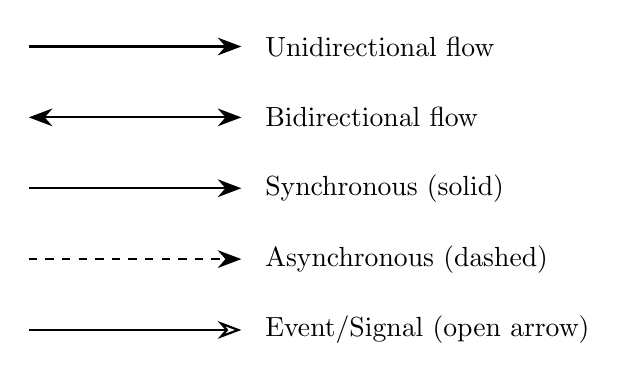
\begin{tikzpicture}[scale=0.9]
    % Unidirectional
    \draw[-{Stealth[length=3mm]}, thick] (0,2) -- (3,2);
    \node[right] at (3.2,2) {Unidirectional flow};
    
    % Bidirectional
    \draw[{Stealth[length=3mm]}-{Stealth[length=3mm]}, thick] (0,1) -- (3,1);
    \node[right] at (3.2,1) {Bidirectional flow};
    
    % Synchronous
    \draw[-{Stealth[length=3mm]}, thick, solid] (0,0) -- (3,0);
    \node[right] at (3.2,0) {Synchronous (solid)};
    
    % Asynchronous
    \draw[-{Stealth[length=3mm]}, thick, dashed] (0,-1) -- (3,-1);
    \node[right] at (3.2,-1) {Asynchronous (dashed)};
    
    % Event
    \draw[-{Stealth[length=3mm, open]}, thick] (0,-2) -- (3,-2);
    \node[right] at (3.2,-2) {Event/Signal (open arrow)};
\end{tikzpicture}
\caption{Flow Type Representations}
\end{figure}

\subsection{Labeling Conventions}

Effective labeling significantly improves diagram comprehension. For entity labels, use noun phrases that identify what the entity is, be specific enough to distinguish similar entities, include role or type qualifiers when helpful, and avoid technical jargon when business context is clearer.

For flow labels, use verb phrases describing what is exchanged or performed, indicate the direction of data or control flow, specify the interaction pattern (request/response, publish/subscribe, etc.), and note protocols or standards when architecturally significant.

\begin{example}
\textbf{Good Labels:}
\begin{itemize}[nosep]
    \item ``Customer'' (not ``User1'')
    \item ``Payment Gateway'' (not ``External System'')
    \item ``Submit Order'' (not ``HTTP POST'')
    \item ``Receive Shipment Notification'' (not ``Message'')
\end{itemize}

\textbf{Poor Labels:}
\begin{itemize}[nosep]
    \item ``Actor A'' (too generic)
    \item ``System'' (ambiguous)
    \item ``Data'' (uninformative)
    \item ``Process'' (vague)
\end{itemize}
\end{example}

\subsection{Diagram Layout Guidelines}

Professional diagram layout follows these principles. First, center the SUD to give it visual prominence. Second, group related entities by placing similar external entities near each other. Third, minimize crossing by arranging entities and flows to reduce line crossings. Fourth, use consistent spacing to maintain uniform distances between elements. Fifth, align elements to use grid alignment for a clean appearance. Sixth, consider reading order by placing primary actors on the left and downstream systems on the right. Seventh, maintain balance by distributing entities around the SUD for visual equilibrium.

%==============================================================================
\section{External Entity Classification and Documentation}
%==============================================================================

\subsection{Entity Type Taxonomy}

External entities can be classified into several primary categories, each with distinct characteristics affecting how they should be documented and managed:

\subsubsection{Human Actors}

Human actors are people who interact directly with the system. Documentation should include role or persona name, organizational affiliation, interaction frequency (daily, weekly, occasional), primary tasks performed, skill level and training requirements, and authorization level and access rights.

\begin{longtable}{@{}>{\raggedright\arraybackslash}p{3cm} p{4cm} p{6cm}@{}}
\caption{Human Actor Documentation Template} \\
\toprule
\textbf{Attribute} & \textbf{Description} & \textbf{Example} \\
\midrule
\endfirsthead
\toprule
\textbf{Attribute} & \textbf{Description} & \textbf{Example} \\
\midrule
\endhead
\midrule
\multicolumn{3}{r}{\textit{Continued on next page}} \\
\endfoot
\bottomrule
\endlastfoot
Actor Name & Official role designation & Sales Representative \\
Organization & Company or department & Acme Corp, Sales Division \\
Interaction Mode & How they access the system & Web browser, mobile app \\
Frequency & How often they interact & Daily, 20-50 transactions \\
Primary Tasks & Main activities performed & Create quotes, process orders \\
Authorization & Access level & Read customer data, write orders \\
Volume & Number of concurrent users & 500 peak, 200 average \\
Location & Geographic distribution & North America, Europe \\
\end{longtable}

\subsubsection{External Systems}

External systems are software applications or services outside the system boundary that exchange data or control with the SUD. Documentation should include system name and version, system owner and contact, interface type (API, file transfer, messaging), data exchanged, SLA requirements, and dependency criticality.

\begin{longtable}{@{}>{\raggedright\arraybackslash}p{3cm} p{4cm} p{6cm}@{}}
\caption{External System Documentation Template} \\
\toprule
\textbf{Attribute} & \textbf{Description} & \textbf{Example} \\
\midrule
\endfirsthead
\toprule
\textbf{Attribute} & \textbf{Description} & \textbf{Example} \\
\midrule
\endhead
\midrule
\multicolumn{3}{r}{\textit{Continued on next page}} \\
\endfoot
\bottomrule
\endlastfoot
System Name & Official name and version & SAP ERP 6.0 EhP8 \\
Owner & Responsible organization & Finance IT Team \\
Interface Type & Integration mechanism & REST API, SOAP, FTP \\
Protocol & Communication protocol & HTTPS, SFTP, AMQP \\
Data Format & Message/file format & JSON, XML, CSV \\
Authentication & Security mechanism & OAuth 2.0, API Key \\
SLA & Service level agreement & 99.9\% availability, 200ms latency \\
Criticality & Business impact if unavailable & High---blocks order processing \\
\end{longtable}

\subsubsection{Hardware Devices}

Hardware devices are physical equipment that interfaces with the system, including IoT devices, sensors, controllers, and specialized hardware. Documentation should include device type and model, communication protocol, data generation rate, deployment location, and maintenance requirements.

\subsubsection{External Organizations}

External organizations are business entities that have a relationship with the system, such as partners, vendors, regulatory bodies, or customers as organizations. Documentation should include organization name, relationship type, contractual obligations, communication channels, and compliance requirements.

\subsection{Entity Documentation Table}

The following comprehensive table format captures essential information about each external entity:

\setlength{\extrarowheight}{4pt}
\begin{longtable}{@{}>{\bfseries\raggedright\arraybackslash}p{2.5cm} p{2cm} p{2.5cm} p{5.5cm}@{}}
\caption{External Entity Registry Template} \\
\toprule
\textbf{Entity Name} & \textbf{Type} & \textbf{Criticality} & \textbf{Description / Responsibilities} \\
\midrule
\endfirsthead
\toprule
\textbf{Entity Name} & \textbf{Type} & \textbf{Criticality} & \textbf{Description / Responsibilities} \\
\midrule
\endhead
\midrule
\multicolumn{4}{r}{\textit{Continued on next page}} \\
\endfoot
\bottomrule
\endlastfoot
Customer & Human Actor & High & End users who browse products, place orders, and track deliveries. Primary revenue-generating interaction point. \\
Administrator & Human Actor & Medium & Internal staff who manage product catalog, user accounts, and system configuration. \\
Payment Gateway & External System & Critical & Third-party service (Stripe/PayPal) processing all financial transactions. Single point of failure for revenue. \\
Inventory System & External System & High & ERP system maintaining authoritative inventory levels. Source of truth for availability. \\
Shipping Provider & External System & High & FedEx/UPS APIs for rate calculation, label generation, and tracking. \\
Mobile Device & Device & Medium & iOS/Android devices running the customer mobile application. \\
POS Terminal & Device & High & Point-of-sale hardware in retail locations integrating with the system. \\
Regulatory Body & Organization & Low & Government agencies requiring compliance reporting and audits. \\
\end{longtable}

\subsection{Entity Cardinality and Multiplicity}

When documenting external entities, consider their cardinality---how many instances of each entity type exist and interact with the system. This affects architectural decisions around scalability, session management, and resource allocation.

Single instance entities are unique external entities where only one exists (for example, a specific ERP system or a single payment processor). Multiple instance entities are categories where many individual instances exist (for example, customers, where thousands may interact). Pooled entities are instances that may be treated as interchangeable (for example, load-balanced API endpoints). Hierarchical entities are instances with parent-child relationships (for example, organizations with departments with users).

Document cardinality using notation like: ``Customer [1..*]'' for one or more customers, ``Payment Gateway [1]'' for exactly one payment gateway, ``Shipping Provider [1..3]'' for one to three shipping providers, and ``IoT Sensor [100..10000]'' for 100 to 10,000 sensors.

%==============================================================================
\section{Interactions and Interfaces}
%==============================================================================

\subsection{Interaction Classification}

Interactions between the SUD and external entities can be classified along several dimensions:

\subsubsection{By Direction}

Inbound interactions flow from an external entity to the SUD, such as requests, commands, data submissions, and events that the SUD must handle. Outbound interactions flow from the SUD to an external entity, such as responses, notifications, data exports, and commands to external systems. Bidirectional interactions involve exchange in both directions, typically request-response patterns or ongoing conversations.

\subsubsection{By Timing}

Synchronous interactions require the initiator to wait for a response before proceeding. Asynchronous interactions allow the initiator to continue without waiting, with responses handled separately. Real-time interactions require immediate processing and response within tight time constraints. Batch interactions involve periodic processing of accumulated data.

\subsubsection{By Pattern}

Request-response patterns are classic client-server interactions where one party requests and another responds. Publish-subscribe patterns involve the SUD or external entities publishing events that interested parties receive. Command patterns involve one party issuing commands that another party executes. Query patterns are read-only requests for information without side effects. Stream patterns involve continuous data flow rather than discrete messages.

\subsection{Interaction Documentation}

Each significant interaction should be documented with sufficient detail to support interface design and implementation:

\setlength{\extrarowheight}{4pt}
\begin{longtable}{@{}>{\bfseries\raggedright\arraybackslash}p{1.8cm} p{1.8cm} p{2.2cm} p{2cm} p{4.5cm}@{}}
\caption{Interaction Registry Template} \\
\toprule
\textbf{From} & \textbf{To} & \textbf{Interaction} & \textbf{Pattern} & \textbf{Description / Requirements} \\
\midrule
\endfirsthead
\toprule
\textbf{From} & \textbf{To} & \textbf{Interaction} & \textbf{Pattern} & \textbf{Description / Requirements} \\
\midrule
\endhead
\midrule
\multicolumn{5}{r}{\textit{Continued on next page}} \\
\endfoot
\bottomrule
\endlastfoot
Customer & SUD & Browse Catalog & Sync Req/Resp & HTTP GET requests for product listings; must support 1000 req/sec with <200ms response \\
Customer & SUD & Submit Order & Sync Req/Resp & HTTP POST with order details; requires transactional integrity and confirmation \\
SUD & Payment Gateway & Process Payment & Sync Req/Resp & REST API call with card details; PCI-DSS compliant; timeout 30 seconds \\
SUD & Inventory System & Check Availability & Sync Query & Real-time inventory query; cached locally with 5-minute TTL \\
SUD & Shipping Provider & Request Rates & Sync Req/Resp & Batch rate requests; acceptable latency up to 5 seconds \\
SUD & Customer & Order Confirmation & Async Event & Email/SMS notification; delivery within 1 minute of order completion \\
Inventory System & SUD & Stock Update & Async Pub/Sub & Real-time inventory changes via message queue; must handle 100 msgs/sec \\
IoT Sensor & SUD & Telemetry Data & Stream & Continuous sensor readings every 100ms; UDP protocol; lossy acceptable \\
\end{longtable}

\subsection{Interface Specification Summary}

For each external interface, create a summary specification that can serve as input to detailed interface design:

\begin{tcolorbox}[colback=lightgray, colframe=flowcolor, title=Interface Specification Template]
\textbf{Interface Name:} Unique identifier for the interface

\textbf{External Entity:} The external entity this interface connects to

\textbf{Direction:} Inbound / Outbound / Bidirectional

\textbf{Protocol:} Communication protocol (HTTP, AMQP, gRPC, etc.)

\textbf{Data Format:} Message format (JSON, XML, Protobuf, etc.)

\textbf{Authentication:} Security mechanism (OAuth, API key, mTLS, etc.)

\textbf{Operations:} List of operations/endpoints exposed or consumed

\textbf{Data Elements:} Key data entities exchanged

\textbf{Volume:} Expected transaction volume (requests/sec, MB/day)

\textbf{Latency:} Response time requirements

\textbf{Availability:} Uptime requirements and failure handling

\textbf{Error Handling:} How errors are communicated and handled

\textbf{Versioning:} Strategy for interface evolution

\textbf{Documentation:} Link to detailed API/interface documentation
\end{tcolorbox}

\subsection{Data Flow Specifications}

For significant data flows, document the data elements exchanged:

\begin{longtable}{@{}>{\raggedright\arraybackslash}p{2.5cm} p{3cm} p{3cm} p{4cm}@{}}
\caption{Data Flow Specification Template} \\
\toprule
\textbf{Flow Name} & \textbf{Source $\rightarrow$ Target} & \textbf{Data Elements} & \textbf{Constraints} \\
\midrule
\endfirsthead
\toprule
\textbf{Flow Name} & \textbf{Source $\rightarrow$ Target} & \textbf{Data Elements} & \textbf{Constraints} \\
\midrule
\endhead
\midrule
\multicolumn{4}{r}{\textit{Continued on next page}} \\
\endfoot
\bottomrule
\endlastfoot
Order Submission & Customer $\rightarrow$ SUD & Customer ID, Product IDs, Quantities, Shipping Address, Payment Token & Authenticated; max 100 line items; valid address required \\
Payment Request & SUD $\rightarrow$ Payment Gateway & Order ID, Amount, Currency, Payment Token, Merchant ID & PCI-DSS compliant; amount > 0; supported currencies only \\
Inventory Query & SUD $\rightarrow$ Inventory System & Product IDs, Warehouse ID & Max 50 products per query; warehouse must be active \\
Shipment Notification & Shipping Provider $\rightarrow$ SUD & Order ID, Tracking Number, Carrier, Status, Timestamp & Webhook callback; idempotent processing required \\
\end{longtable}

%==============================================================================
\section{Context Diagram Construction}
%==============================================================================

\subsection{Step-by-Step Process}

Creating an effective context diagram follows a systematic process:

\subsubsection{Step 1: Define the System Mission}

Begin by articulating the system's purpose in one or two sentences. This mission statement guides all subsequent boundary and scope decisions. Ensure stakeholder agreement on the mission before proceeding. The mission should answer: What problem does this system solve? Who benefits from this system? What value does it provide?

\subsubsection{Step 2: Identify Stakeholders}

List all individuals, groups, and organizations with an interest in the system. Stakeholders include direct users who interact with the system daily, indirect users who benefit from system outputs, system owners responsible for the system's success, operators who maintain and support the system, external partners who integrate with the system, and regulatory bodies who impose compliance requirements.

\subsubsection{Step 3: Enumerate External Entities}

For each stakeholder, identify the external entities that will appear in the context diagram. Apply these criteria: the entity must be external, meaning outside the system boundary and not part of the system being designed. The entity must be interactive, meaning it exchanges data, control, or events with the system. The entity must be significant, meaning the interaction is architecturally relevant and not a trivial detail. Aggregate similar entities: if many individuals play the same role (for example, customers), represent them as a single entity type.

\subsubsection{Step 4: Map Interactions}

For each external entity, identify all significant interactions. Consider what data the entity sends to the system, what data the entity receives from the system, what events or notifications flow between them, what commands or requests are exchanged, and what the triggering conditions and frequencies are.

\subsubsection{Step 5: Establish Boundaries}

Explicitly define what is inside versus outside the system boundary. For each potential element, ask: Is this element the responsibility of this system? Is this element under the control of this development effort? Is this element within the scope of this project? Document boundary decisions and their rationale.

\subsubsection{Step 6: Draft the Diagram}

Create an initial diagram following the notation conventions. Place the SUD centrally and position external entities around it. Draw interactions as flows between entities and the SUD. Label all elements and flows clearly.

\subsubsection{Step 7: Validate with Stakeholders}

Review the diagram with key stakeholders. Verify all external entities are represented, no internal components are shown as external, all significant interactions are captured, labels are clear and meaningful, and the boundary matches stakeholder expectations.

\subsubsection{Step 8: Document Supporting Details}

Complete the documentation with entity descriptions, interaction specifications, assumptions, dependencies, and quality attribute considerations.

\subsection{Example Context Diagram}

The following example illustrates a context diagram for an e-commerce order management system:

\begin{figure}[H]
\centering
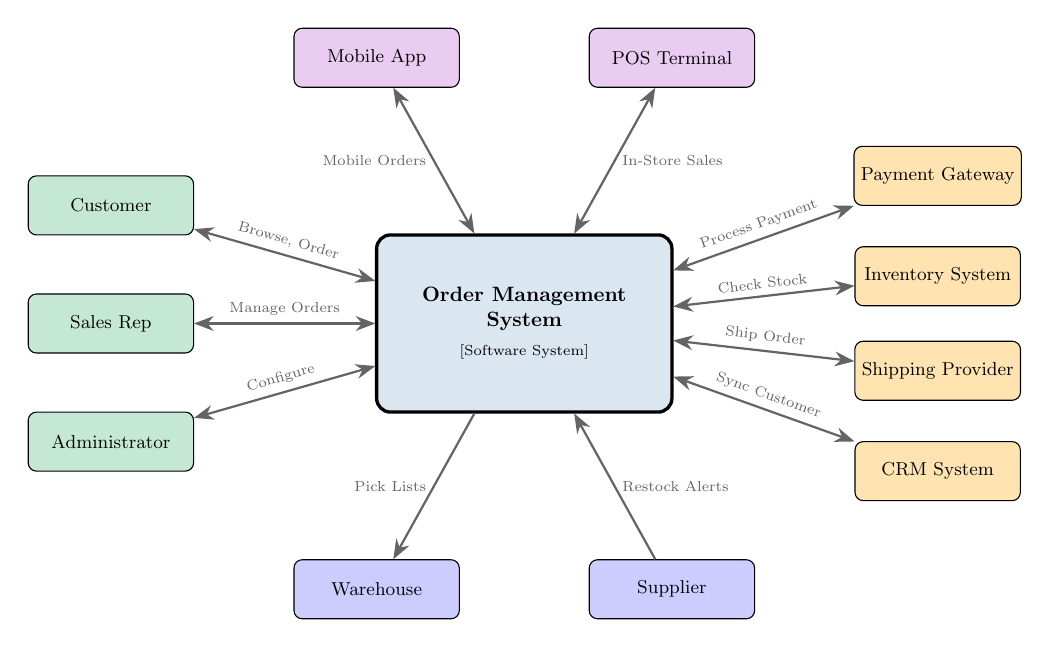
\begin{tikzpicture}[
    scale=0.75,
    transform shape,
    sud/.style={draw, very thick, fill=sudcolor!20, minimum width=5cm, minimum height=3cm, rounded corners=5pt},
    actor/.style={draw, fill=actorcolor!30, minimum width=2.8cm, minimum height=1cm, rounded corners=3pt, font=\small},
    system/.style={draw, fill=systemcolor!30, minimum width=2.8cm, minimum height=1cm, rounded corners=3pt, font=\small},
    device/.style={draw, fill=devicecolor!30, minimum width=2.8cm, minimum height=1cm, rounded corners=3pt, font=\small},
    org/.style={draw, fill=blue!20, minimum width=2.8cm, minimum height=1cm, rounded corners=3pt, font=\small},
    flow/.style={-{Stealth[length=2.5mm]}, thick, flowcolor},
    biflow/.style={{Stealth[length=2.5mm]}-{Stealth[length=2.5mm]}, thick, flowcolor},
    label/.style={font=\scriptsize, flowcolor}
]
    % SUD
    \node[sud] (sud) at (0,0) {%
        \begin{tabular}{c}
            \textbf{Order Management}\\
            \textbf{System}\\[2pt]
            \scriptsize [Software System]
        \end{tabular}
    };
    
    % Human Actors (Left)
    \node[actor] (customer) at (-7,2) {Customer};
    \node[actor] (sales) at (-7,0) {Sales Rep};
    \node[actor] (admin) at (-7,-2) {Administrator};
    
    % External Systems (Right)
    \node[system] (payment) at (7,2.5) {Payment Gateway};
    \node[system] (inventory) at (7,0.8) {Inventory System};
    \node[system] (shipping) at (7,-0.8) {Shipping Provider};
    \node[system] (crm) at (7,-2.5) {CRM System};
    
    % Devices (Top)
    \node[device] (mobile) at (-2.5,4.5) {Mobile App};
    \node[device] (pos) at (2.5,4.5) {POS Terminal};
    
    % Organizations (Bottom)
    \node[org] (warehouse) at (-2.5,-4.5) {Warehouse};
    \node[org] (supplier) at (2.5,-4.5) {Supplier};
    
    % Flows from actors
    \draw[biflow] (customer) -- node[label, above, sloped] {Browse, Order} (sud);
    \draw[biflow] (sales) -- node[label, above, sloped] {Manage Orders} (sud);
    \draw[biflow] (admin) -- node[label, above, sloped] {Configure} (sud);
    
    % Flows to systems
    \draw[biflow] (sud) -- node[label, above, sloped] {Process Payment} (payment);
    \draw[biflow] (sud) -- node[label, above, sloped] {Check Stock} (inventory);
    \draw[biflow] (sud) -- node[label, above, sloped] {Ship Order} (shipping);
    \draw[biflow] (sud) -- node[label, above, sloped] {Sync Customer} (crm);
    
    % Flows from devices
    \draw[biflow] (mobile) -- node[label, left] {Mobile Orders} (sud);
    \draw[biflow] (pos) -- node[label, right] {In-Store Sales} (sud);
    
    % Flows from organizations
    \draw[flow] (sud) -- node[label, left] {Pick Lists} (warehouse);
    \draw[flow] (supplier) -- node[label, right] {Restock Alerts} (sud);
    
\end{tikzpicture}
\caption{Example Context Diagram: Order Management System}
\label{fig:example-context}
\end{figure}

%==============================================================================
\section{Assumptions and Dependencies}
%==============================================================================

\subsection{Documenting Assumptions}

Assumptions are conditions believed to be true that influence architectural decisions. Undocumented assumptions are a leading cause of project failures. For each assumption, document the assumption statement describing what is assumed to be true, the basis or evidence supporting this assumption, the impact describing what happens if the assumption proves false, the owner responsible for validating the assumption, and the validation date when it was or will be confirmed.

\subsubsection{Categories of Assumptions}

Environmental assumptions concern the operating context of the system, such as network connectivity being consistently available with latency under 100ms or user browsers supporting HTML5 and JavaScript ES6+.

Organizational assumptions concern people and processes, such as business users being available for UAT within 2 weeks of release or IT operations providing 24/7 monitoring and incident response.

Technical assumptions concern technology platforms and capabilities, such as the cloud provider guaranteeing 99.95\% uptime for compute services or database connection pooling supporting 500 concurrent connections.

External system assumptions concern systems outside the boundary, such as the payment gateway supporting tokenization for PCI compliance or the legacy ERP exposing a stable API for inventory queries.

\subsection{Assumptions Documentation Template}

\begin{longtable}{@{}>{\raggedright\arraybackslash}p{0.5cm} p{4cm} p{2cm} p{3cm} p{2.5cm}@{}}
\caption{Assumptions Registry} \\
\toprule
\textbf{ID} & \textbf{Assumption} & \textbf{Category} & \textbf{Impact if False} & \textbf{Validation} \\
\midrule
\endfirsthead
\toprule
\textbf{ID} & \textbf{Assumption} & \textbf{Category} & \textbf{Impact if False} & \textbf{Validation} \\
\midrule
\endhead
\midrule
\multicolumn{5}{r}{\textit{Continued on next page}} \\
\endfoot
\bottomrule
\endlastfoot
A1 & Payment gateway supports OAuth 2.0 for authentication & Technical & Must implement alternative auth; 2-week delay & Confirmed via API docs \\
A2 & Average order contains fewer than 50 line items & Business & Performance requirements must be revised & Pending data analysis \\
A3 & Inventory system available 99.9\% of business hours & External & Must implement caching/fallback & SLA review pending \\
A4 & Users have broadband internet (>5 Mbps) & Environmental & Must optimize for low bandwidth & User survey Q2 \\
A5 & Legal review completed before PII data collection & Organizational & Launch delay; compliance risk & Legal team confirmed \\
\end{longtable}

\subsection{Documenting Dependencies}

Dependencies are external factors the system relies upon that are outside the team's control. Unlike assumptions (believed to be true), dependencies are known requirements on external parties.

\subsubsection{Dependency Categories}

Runtime dependencies are required for the system to operate. Examples include external API availability for core functions, network connectivity between components, and database service availability.

Build-time dependencies are required to build and deploy the system. Examples include CI/CD pipeline availability, artifact repository access, and deployment environment provisioning.

Development dependencies are required for development activities. Examples include development tool licenses, test environment access, and third-party SDK availability.

Organizational dependencies are required from people and processes. Examples include stakeholder availability for decisions, SME access for requirements clarification, and approval processes for production releases.

\subsection{Dependencies Documentation Template}

\begin{longtable}{@{}>{\raggedright\arraybackslash}p{0.5cm} p{3cm} p{2.5cm} p{3.5cm} p{2.5cm}@{}}
\caption{Dependencies Registry} \\
\toprule
\textbf{ID} & \textbf{Dependency} & \textbf{Provider} & \textbf{Mitigation if Unavailable} & \textbf{Status} \\
\midrule
\endfirsthead
\toprule
\textbf{ID} & \textbf{Dependency} & \textbf{Provider} & \textbf{Mitigation if Unavailable} & \textbf{Status} \\
\midrule
\endhead
\midrule
\multicolumn{5}{r}{\textit{Continued on next page}} \\
\endfoot
\bottomrule
\endlastfoot
D1 & Payment processing API & Stripe Inc. & Failover to PayPal backup & Active; SLA in place \\
D2 & Inventory data feed & SAP ERP Team & Local cache with manual sync & Active; API stable \\
D3 & Cloud infrastructure & AWS & Multi-region deployment & Active; Enterprise agreement \\
D4 & SSL certificates & DigiCert & Backup CA identified & Annual renewal Q4 \\
D5 & OAuth identity provider & Okta & Local auth fallback (degraded) & Active; SSO integrated \\
\end{longtable}

\subsection{Dependency Risk Assessment}

For critical dependencies, perform a risk assessment. Consider the probability of unavailability ranging from rare to likely. Consider the impact of unavailability ranging from low (minor inconvenience) to critical (system failure). Consider detectability in terms of how quickly the failure would be detected. Consider recoverability in terms of how quickly normal operation can be restored.

\begin{bestpractice}
For each high-impact dependency, ensure you have identified an alternative approach or fallback, defined monitoring and alerting for dependency health, documented manual procedures if automation fails, and tested failover procedures regularly.
\end{bestpractice}

%==============================================================================
\section{Quality Attribute Considerations}
%==============================================================================

\subsection{Context-Level Quality Attributes}

The system's interactions with its environment significantly impact quality attributes. The context diagram should inform quality attribute analysis in several dimensions.

\subsubsection{Performance}

Cross-boundary interactions often dominate system latency. Consider network latency to external systems, serialization and deserialization overhead, external system response times, and data volume and transfer rates.

Document performance requirements for each external interaction. What is the expected latency? What throughput is required? What is acceptable degradation under load?

\subsubsection{Availability}

System availability depends on the availability of external dependencies. Consider external system uptime guarantees (SLAs), failure modes and their probability, and recovery time objectives (RTO) for each dependency.

For each critical external system, document the expected availability (for example, 99.9\%), the impact on SUD availability if unavailable, failover or degradation strategy, and monitoring and alerting approach.

\subsubsection{Security}

The context diagram defines trust boundaries---the points where trust levels change. Consider which external entities are trusted versus untrusted, what authentication is required at each boundary, what authorization controls are needed, what data must be protected in transit, and what audit logging is required for external interactions.

\begin{figure}[H]
\centering
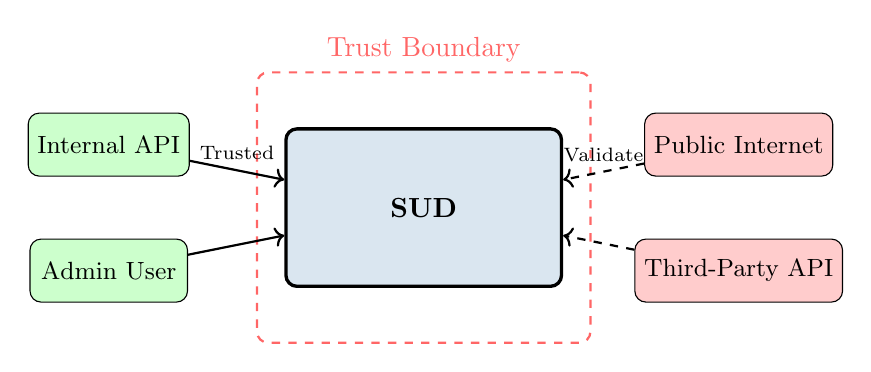
\begin{tikzpicture}[
    scale=0.8,
    trust/.style={draw, dashed, thick, red!60, rounded corners},
    sud/.style={draw, very thick, fill=sudcolor!20, minimum width=3.5cm, minimum height=2cm, rounded corners},
    entity/.style={draw, fill=gray!20, minimum width=2cm, minimum height=0.8cm, rounded corners, font=\small}
]
    % Trust boundary
    \begin{scope}[on background layer]
        \node[trust, fit={(-2.5,-2) (2.5,2)}, label={[red!60]above:Trust Boundary}] {};
    \end{scope}
    
    % SUD
    \node[sud] (sud) at (0,0) {\textbf{SUD}};
    
    % Trusted entities (inside boundary conceptually)
    \node[entity, fill=green!20] (trusted1) at (-5,1) {Internal API};
    \node[entity, fill=green!20] (trusted2) at (-5,-1) {Admin User};
    
    % Untrusted entities (outside boundary)
    \node[entity, fill=red!20] (untrusted1) at (5,1) {Public Internet};
    \node[entity, fill=red!20] (untrusted2) at (5,-1) {Third-Party API};
    
    \draw[->, thick] (trusted1) -- node[above, font=\scriptsize] {Trusted} (sud);
    \draw[->, thick] (trusted2) -- (sud);
    \draw[->, thick, dashed] (untrusted1) -- node[above, font=\scriptsize] {Validate} (sud);
    \draw[->, thick, dashed] (untrusted2) -- (sud);
\end{tikzpicture}
\caption{Trust Boundaries in Context Diagram}
\end{figure}

\subsubsection{Scalability}

External interactions often become bottlenecks under scale. Consider external system rate limits, connection pool limitations, data volume growth projections, and geographic distribution requirements.

\subsubsection{Reliability}

External system failures will occur. Consider graceful degradation when external systems fail, retry and circuit-breaker patterns, idempotency requirements for retryable operations, and data consistency across system boundaries.

\subsection{Quality Attribute Scenarios}

Document quality attribute requirements as concrete scenarios tied to external interactions:

\begin{longtable}{@{}>{\raggedright\arraybackslash}p{2cm} p{3.5cm} p{3.5cm} p{3.5cm}@{}}
\caption{Quality Attribute Scenarios} \\
\toprule
\textbf{Attribute} & \textbf{Scenario} & \textbf{Measure} & \textbf{Response} \\
\midrule
\endfirsthead
\toprule
\textbf{Attribute} & \textbf{Scenario} & \textbf{Measure} & \textbf{Response} \\
\midrule
\endhead
\midrule
\multicolumn{4}{r}{\textit{Continued on next page}} \\
\endfoot
\bottomrule
\endlastfoot
Performance & Customer submits order during peak load & Response time <2 seconds at 95th percentile & Queue requests; scale horizontally \\
Availability & Payment gateway becomes unreachable & System remains available for browsing and cart management & Circuit breaker; retry with backoff \\
Security & Attacker attempts injection via API & All attacks blocked; no data exposure & Input validation; parameterized queries \\
Scalability & Holiday traffic increases 10x normal & System handles load without degradation & Auto-scaling; CDN caching \\
Reliability & Network partition between SUD and inventory system & Orders continue with cached inventory; reconcile later & Local cache; eventual consistency \\
\end{longtable}

%==============================================================================
\section{Regulatory and Compliance Considerations}
%==============================================================================

\subsection{Compliance Impact on Context}

Regulatory requirements often impose constraints on system boundaries and external interactions. Common regulatory frameworks affecting system context include GDPR (General Data Protection Regulation) governing data protection and privacy for EU residents, HIPAA (Health Insurance Portability and Accountability Act) governing healthcare data in the US, PCI-DSS (Payment Card Industry Data Security Standard) governing payment card data handling, SOX (Sarbanes-Oxley Act) governing financial reporting and controls, and SOC 2 (Service Organization Control 2) governing security, availability, and confidentiality.

\subsection{Compliance Documentation}

For each applicable regulation, document the regulation name and jurisdiction, applicable data types within the system, external entities handling regulated data, required controls for external interactions, audit and reporting requirements, and data residency constraints.

\begin{longtable}{@{}>{\raggedright\arraybackslash}p{2cm} p{2.5cm} p{3cm} p{5cm}@{}}
\caption{Compliance Requirements Matrix} \\
\toprule
\textbf{Regulation} & \textbf{Data Types} & \textbf{External Entities} & \textbf{Required Controls} \\
\midrule
\endfirsthead
\toprule
\textbf{Regulation} & \textbf{Data Types} & \textbf{External Entities} & \textbf{Required Controls} \\
\midrule
\endhead
\midrule
\multicolumn{4}{r}{\textit{Continued on next page}} \\
\endfoot
\bottomrule
\endlastfoot
GDPR & Customer PII & CRM System, Analytics Provider & Consent management; data minimization; right to erasure; DPA with processors \\
PCI-DSS & Payment card data & Payment Gateway & Tokenization; encrypted transmission; no local storage of card numbers \\
SOC 2 & All customer data & Cloud Infrastructure, Backup Provider & Access controls; encryption; monitoring; incident response \\
\end{longtable}

\subsection{Data Flow Compliance Annotations}

Annotate data flows in the context diagram with compliance requirements. For each flow involving regulated data, document the data classification level, encryption requirements (in transit, at rest), access control requirements, retention and deletion requirements, and audit logging requirements.

%==============================================================================
\section{Domain-Specific Context Patterns}
%==============================================================================

\subsection{Enterprise Application Context}

Enterprise applications typically integrate with numerous internal and external systems. Common external entities include ERP systems (SAP, Oracle) as source of financial and operational data, identity providers (Active Directory, Okta) for authentication and authorization, enterprise service buses or API gateways as integration middleware, data warehouses and business intelligence systems as analytics destinations, and legacy systems requiring integration adapters.

\begin{bestpractice}
For enterprise contexts, pay special attention to data ownership (which system is the master for each data entity), integration patterns (synchronous vs. event-driven), and organizational boundaries (different teams owning different systems).
\end{bestpractice}

\subsection{Cloud-Native Application Context}

Cloud-native systems have unique context considerations. Common external entities include cloud platform services (compute, storage, messaging), managed databases (RDS, Cloud SQL, Cosmos DB), container orchestration platforms (Kubernetes services), observability platforms (monitoring, logging, tracing), and CDN and edge services.

Key considerations for cloud-native contexts include service mesh boundaries (what's inside vs. outside the mesh), multi-region and multi-cloud deployments, serverless function integration, and managed service dependencies.

\subsection{IoT System Context}

IoT systems interact with numerous devices and gateways. Common external entities include edge devices (sensors, actuators, controllers), edge gateways (aggregating device data), device management platforms, time-series databases, analytics and ML platforms, and mobile applications for device control.

Key considerations for IoT contexts include device provisioning and lifecycle, intermittent connectivity handling, data volume and velocity, and device security and authentication.

\subsection{Mobile Application Context}

Mobile applications have specific context requirements. Common external entities include backend API services, push notification services (APNs, FCM), analytics and crash reporting services, app stores (deployment and updates), and device capabilities (camera, GPS, biometrics).

Key considerations for mobile contexts include offline operation capability, network variability handling, app store compliance, and device fragmentation.

%==============================================================================
\section{Context Diagram Maintenance}
%==============================================================================

\subsection{Living Documentation}

The context diagram should be maintained as a living document throughout the system lifecycle. Keeping it current ensures new team members can quickly understand system scope, architectural decisions remain grounded in documented context, integration changes are properly evaluated, and compliance audits have accurate documentation.

\subsection{Change Management Process}

When changes affect the system context, follow this process. First, identify the change such as new external entity, modified interaction, or boundary change. Second, assess the impact on architecture, interfaces, security, and compliance. Third, update the diagram and supporting documentation. Fourth, review changes with stakeholders. Fifth, communicate the changes to affected teams. Sixth, verify that implementation matches updated documentation.

\subsection{Version Control and Traceability}

Maintain version control for context documentation. Track the version number using semantic versioning (MAJOR.MINOR.PATCH), the change date, the author, a change summary, and traceability by linking changes to requirements, decisions, or incidents.

\begin{longtable}{@{}>{\raggedright\arraybackslash}p{1.5cm} p{2cm} p{2cm} p{7cm}@{}}
\caption{Context Diagram Version History} \\
\toprule
\textbf{Version} & \textbf{Date} & \textbf{Author} & \textbf{Changes} \\
\midrule
\endfirsthead
\toprule
\textbf{Version} & \textbf{Date} & \textbf{Author} & \textbf{Changes} \\
\midrule
\endhead
\midrule
\multicolumn{4}{r}{\textit{Continued on next page}} \\
\endfoot
\bottomrule
\endlastfoot
1.0.0 & 2024-01-15 & J. Smith & Initial context diagram and documentation \\
1.1.0 & 2024-03-22 & A. Jones & Added mobile app as external entity; updated interaction table \\
1.2.0 & 2024-06-10 & J. Smith & Added compliance section for GDPR requirements \\
2.0.0 & 2024-09-01 & B. Chen & Major revision: new payment provider; removed legacy ERP integration \\
\end{longtable}

%==============================================================================
\section{Common Pitfalls and Anti-patterns}
%==============================================================================

\subsection{Diagram Anti-patterns}

\begin{warning}
Avoid these common mistakes when creating context diagrams:

\textbf{Exploded Context:} Including too much internal detail that belongs in lower-level diagrams. The SUD should remain a black box at this level.

\textbf{Missing Actors:} Forgetting to include operational roles (administrators, operators, support staff) or automated actors (schedulers, monitors).

\textbf{Technology Focus:} Labeling entities with technology names (``Oracle Database'') rather than business roles (``Customer Data Store'').

\textbf{Inconsistent Abstraction:} Mixing high-level entities (``Partner Organization'') with low-level details (``REST API Endpoint'').

\textbf{Missing Flows:} Showing entities without indicating what data or control flows between them and the SUD.

\textbf{Unlabeled Flows:} Drawing arrows without describing what they represent.

\textbf{Boundary Ambiguity:} Not clearly distinguishing what's inside versus outside the system boundary.
\end{warning}

\subsection{Documentation Anti-patterns}

\begin{warning}
Avoid these documentation mistakes:

\textbf{Stale Documentation:} Creating the context diagram once and never updating it as the system evolves.

\textbf{Isolated Diagram:} Presenting the diagram without supporting documentation of entities, interactions, and assumptions.

\textbf{Disconnected from Reality:} Documenting the intended design rather than the actual implementation.

\textbf{Missing Rationale:} Not explaining why boundaries were drawn where they are.

\textbf{Assumed Knowledge:} Using acronyms, jargon, or references without definition.

\textbf{No Validation:} Not reviewing the diagram with stakeholders who know the actual system context.
\end{warning}

%==============================================================================
\section{Tooling and Automation}
%==============================================================================

\subsection{Diagramming Tools}

Several tools support context diagram creation. General-purpose diagramming tools include Lucidchart (web-based, collaborative), draw.io or diagrams.net (free, open-source), Microsoft Visio (enterprise standard), and Miro (collaborative whiteboarding). Architecture-specific tools include Structurizr (C4 model support with DSL), Archi (ArchiMate modeling), Enterprise Architect (comprehensive UML/SysML), and PlantUML (text-based diagrams).

\subsection{Diagram-as-Code}

Modern practices favor diagram-as-code approaches for version control, reproducibility, and automation:

\begin{example}
\textbf{Structurizr DSL Example:}
\begin{verbatim}
workspace {
    model {
        customer = person "Customer" "End user"
        admin = person "Administrator" "System admin"
        
        orderSystem = softwareSystem "Order Management" {
            description "Manages customer orders"
        }
        
        paymentGateway = softwareSystem "Payment Gateway" {
            description "Processes payments"
            tags "External"
        }
        
        customer -> orderSystem "Places orders"
        admin -> orderSystem "Manages configuration"
        orderSystem -> paymentGateway "Processes payments"
    }
    
    views {
        systemContext orderSystem "Context" {
            include *
            autoLayout
        }
    }
}
\end{verbatim}
\end{example}

\subsection{Documentation Integration}

Integrate context diagrams with other documentation through linked documentation that connects the diagram to detailed interface specifications, cross-referencing that maps diagram elements to requirements, decision records, and test cases, and automated updates that generate or update documentation from structured diagram data.

%==============================================================================
\section{Review Checklist}
%==============================================================================

Use this checklist to validate context diagram completeness and quality:

\subsection{Diagram Completeness}

\begin{itemize}[leftmargin=2cm]
    \item[$\square$] SUD is clearly identified and labeled
    \item[$\square$] All human actors are represented
    \item[$\square$] All external systems are represented
    \item[$\square$] All devices and hardware interfaces are represented
    \item[$\square$] All external organizations are represented
    \item[$\square$] All significant data flows are shown
    \item[$\square$] All significant control flows are shown
    \item[$\square$] Flow directions are indicated
    \item[$\square$] Flows are labeled with meaningful descriptions
    \item[$\square$] Entity types are visually distinguished
\end{itemize}

\subsection{Boundary Definition}

\begin{itemize}[leftmargin=2cm]
    \item[$\square$] System boundary is explicitly defined
    \item[$\square$] In-scope elements are documented
    \item[$\square$] Out-of-scope elements are documented
    \item[$\square$] Boundary rationale is explained
    \item[$\square$] No internal components shown as external
    \item[$\square$] No external systems shown as internal
\end{itemize}

\subsection{Documentation Quality}

\begin{itemize}[leftmargin=2cm]
    \item[$\square$] Each external entity is documented with description
    \item[$\square$] Each interaction is documented with details
    \item[$\square$] Assumptions are documented and attributed
    \item[$\square$] Dependencies are documented with mitigation
    \item[$\square$] Quality attribute considerations are addressed
    \item[$\square$] Compliance requirements are identified
    \item[$\square$] Version history is maintained
\end{itemize}

\subsection{Stakeholder Validation}

\begin{itemize}[leftmargin=2cm]
    \item[$\square$] Reviewed with system owner/sponsor
    \item[$\square$] Reviewed with technical leads
    \item[$\square$] Reviewed with integration teams
    \item[$\square$] Reviewed with operations/support
    \item[$\square$] Reviewed with security/compliance
    \item[$\square$] Feedback incorporated and documented
\end{itemize}

%==============================================================================
\section{Open Issues and Questions}
%==============================================================================

Document unresolved questions, pending decisions, and areas requiring further investigation:

\begin{longtable}{@{}>{\raggedright\arraybackslash}p{0.8cm} p{4cm} p{2.5cm} p{2cm} p{3cm}@{}}
\caption{Open Issues Registry} \\
\toprule
\textbf{ID} & \textbf{Issue/Question} & \textbf{Owner} & \textbf{Due Date} & \textbf{Status} \\
\midrule
\endfirsthead
\toprule
\textbf{ID} & \textbf{Issue/Question} & \textbf{Owner} & \textbf{Due Date} & \textbf{Status} \\
\midrule
\endhead
\midrule
\multicolumn{5}{r}{\textit{Continued on next page}} \\
\endfoot
\bottomrule
\endlastfoot
OI-1 & Confirm API versioning strategy for payment gateway integration & Tech Lead & 2024-02-15 & In Progress \\
OI-2 & Determine if mobile app is in-scope for Phase 1 & Product Owner & 2024-02-01 & Pending Decision \\
OI-3 & Clarify data ownership for shared customer records with CRM & Data Architect & 2024-02-20 & Under Discussion \\
OI-4 & Validate availability SLA assumptions with cloud provider & Ops Lead & 2024-02-10 & Scheduled \\
OI-5 & Identify additional compliance requirements for EU expansion & Legal/Compliance & 2024-03-01 & Not Started \\
\end{longtable}

%==============================================================================
\section{Appendix A: Notation Quick Reference}
%==============================================================================

\begin{figure}[H]
\centering
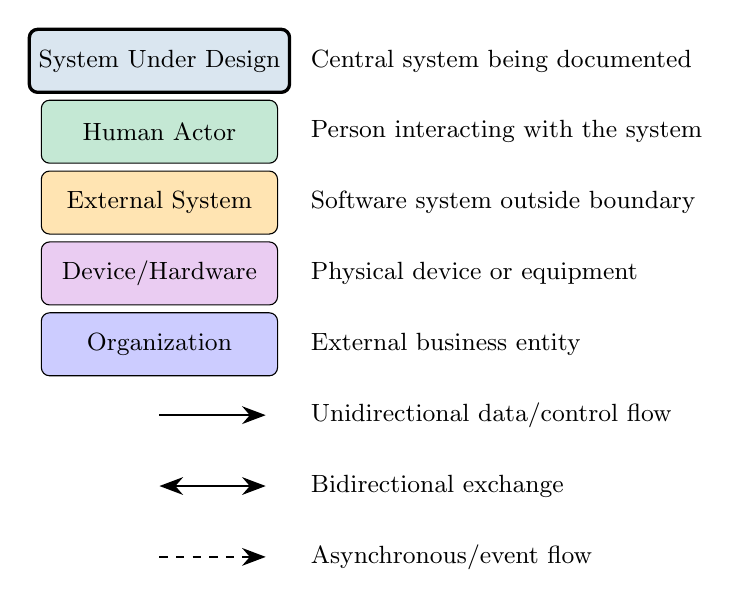
\begin{tikzpicture}[
    scale=0.9,
    box/.style={draw, minimum width=3cm, minimum height=0.8cm, rounded corners=3pt, font=\small}
]
    % Legend items
    \node[box, fill=sudcolor!20, very thick] at (0,4) {System Under Design};
    \node[right, font=\small] at (2,4) {Central system being documented};
    
    \node[box, fill=actorcolor!30] at (0,3) {Human Actor};
    \node[right, font=\small] at (2,3) {Person interacting with the system};
    
    \node[box, fill=systemcolor!30] at (0,2) {External System};
    \node[right, font=\small] at (2,2) {Software system outside boundary};
    
    \node[box, fill=devicecolor!30] at (0,1) {Device/Hardware};
    \node[right, font=\small] at (2,1) {Physical device or equipment};
    
    \node[box, fill=blue!20] at (0,0) {Organization};
    \node[right, font=\small] at (2,0) {External business entity};
    
    % Flow types
    \draw[-{Stealth[length=3mm]}, thick] (0,-1) -- (1.5,-1);
    \node[right, font=\small] at (2,-1) {Unidirectional data/control flow};
    
    \draw[{Stealth[length=3mm]}-{Stealth[length=3mm]}, thick] (0,-2) -- (1.5,-2);
    \node[right, font=\small] at (2,-2) {Bidirectional exchange};
    
    \draw[-{Stealth[length=3mm]}, thick, dashed] (0,-3) -- (1.5,-3);
    \node[right, font=\small] at (2,-3) {Asynchronous/event flow};
\end{tikzpicture}
\caption{Context Diagram Notation Legend}
\end{figure}

%==============================================================================
\section{Appendix B: Template Summary}
%==============================================================================

The following page provides a blank template suitable for documenting a new system's context:

\newpage
\begin{center}
\Large\textbf{Context Diagram Documentation Template}
\end{center}

\vspace{0.5cm}

\textbf{System Name:} \hrulefill

\textbf{Version:} \rule{2cm}{0.4pt} \hspace{1cm} \textbf{Date:} \rule{3cm}{0.4pt} \hspace{1cm} \textbf{Author:} \rule{3cm}{0.4pt}

\vspace{0.5cm}

\textbf{System Mission:}
\begin{tcolorbox}[colback=white, height=2cm]
\end{tcolorbox}

\textbf{System Boundary:}
\begin{tcolorbox}[colback=white, height=3cm]
\textbf{In-Scope:}\\[2cm]
\textbf{Out-of-Scope:}
\end{tcolorbox}

\textbf{Context Diagram:}
\begin{tcolorbox}[colback=white, height=7cm]
\centering\textit{[Insert diagram here]}
\end{tcolorbox}

\textbf{External Entities:}
\begin{tcolorbox}[colback=white, height=4cm]
\begin{tabular}{p{3cm} p{3cm} p{6cm}}
\textbf{Entity} & \textbf{Type} & \textbf{Description} \\
\hline
& & \\
& & \\
& & \\
\end{tabular}
\end{tcolorbox}

%==============================================================================
\section{Appendix C: Glossary}
%==============================================================================

\begin{description}[leftmargin=3cm, style=nextline]
    \item[Actor] An external entity, typically human, that interacts with the system
    \item[Boundary] The dividing line between what is inside and outside the system
    \item[C4 Model] A hierarchical approach to software architecture diagramming (Context, Container, Component, Code)
    \item[Context Diagram] A high-level view showing the system and its external environment
    \item[Data Flow] The movement of data between the system and external entities
    \item[Dependency] An external factor the system relies upon for correct operation
    \item[External Entity] Any person, system, device, or organization outside the system boundary
    \item[Interface] The point of interaction between the system and an external entity
    \item[SLA] Service Level Agreement; contractual performance commitments
    \item[SUD] System Under Design; the system being documented
    \item[Trust Boundary] A point where security trust levels change
\end{description}

%==============================================================================
\section{References}
%==============================================================================

\begin{enumerate}
    \item Bass, L., Clements, P., \& Kazman, R. (2021). \textit{Software Architecture in Practice} (4th ed.). Addison-Wesley.
    
    \item Brown, S. (2018). \textit{The C4 Model for Visualising Software Architecture}. Retrieved from \url{https://c4model.com}
    
    \item Clements, P., et al. (2010). \textit{Documenting Software Architectures: Views and Beyond} (2nd ed.). Addison-Wesley.
    
    \item DeMarco, T. (1979). \textit{Structured Analysis and System Specification}. Yourdon Press.
    
    \item IEEE. (2011). \textit{ISO/IEC/IEEE 42010:2011 Systems and Software Engineering---Architecture Description}.
    
    \item ISO/IEC/IEEE. (2017). \textit{ISO/IEC/IEEE 12207:2017 Systems and Software Engineering---Software Life Cycle Processes}.
    
    \item Rozanski, N., \& Woods, E. (2012). \textit{Software Systems Architecture: Working with Stakeholders Using Viewpoints and Perspectives} (2nd ed.). Addison-Wesley.
    
    \item The Open Group. (2018). \textit{TOGAF Standard, Version 9.2}. Van Haren Publishing.
\end{enumerate}

\end{document}